\documentclass[12pt,a4paper]{article}
\usepackage{amsmath, amssymb, amsfonts, amsthm,latexsym}
\usepackage{graphicx}
\usepackage{verbatim}
\usepackage{multirow}
%\DOTHIS{}{Perhaps readd hyperref which I took out because it
%  generated a warning}
\DeclareMathAlphabet{\mathscr}{OT1}{pzc}{m}{it}

\theoremstyle{definition}

\newtheorem{theorem}{Theorem}[section]
\newtheorem{lemma}[theorem]{Lemma}
\newtheorem*{lemma*}{Lemma}
\newtheorem{definition}[theorem]{Definition}
\newtheorem*{definition*}{Definition}
\newtheorem{notation}[theorem]{Notation}
\newtheorem{example}[theorem]{Example}
\newtheorem{assumption}[theorem]{Assumption}
\newtheorem{note}[theorem]{Note}
\newtheorem{question}[theorem]{Question}
\numberwithin{equation}{section}

\bibliographystyle{plain}
\newtheorem{obs}[theorem]{Observation}
\newtheorem{observation}[theorem]{Observation}
\newtheorem{propos}[theorem]{Proposition}
\newtheorem{defin}{Definition}[section]
\newtheorem{cor}[theorem]{Corollary}
\newtheorem{conjecture}{Conjecture}
\newtheorem{claim}{Claim}
\newtheorem{openproblem}{Open problem}

\newcommand{\insertnote}[3]{\{#2\}[#1: #3]}
%\newcommand{\insertnote}[3]{#2}

\newcommand{\FIXME}{\insertnote{FIXME}}
\newcommand{\TODO}{\insertnote{TODO}}
\newcommand{\DOTHIS}{\insertnote{DOTHIS}}
\newcommand{\EXPLAIN}{\insertnote{EXPLAIN}}
\newcommand{\RON}{\insertnote{RON}}

\renewcommand{\Re}{\operatorname{Re}}
\renewcommand{\Im}{\operatorname{Im}}
\newcommand{\of}{\circ}
\newcommand{\cross}{\times}
\newcommand{\tensor}{\otimes}
\newcommand{\R}{\mathbb{R}}
\newcommand{\minsym}{\wedge}

\newcommand{\ds}{\displaystyle}
\renewcommand{\P}{\mathbb{P}}
\newcommand{\sampled}{X}
\newcommand{\resamplede}{X^{\epsilon}}

\newcommand{\simplex}{\mathcal{S}}

\newcommand{\factor}[2]{\mathcal{F}_{#1 #2}}
\newcommand{\commafactor}[2]{\mathcal{F}_{#1,#2}}
\newcommand{\restrict}[3]{\mathcal{R}_{{#1}{#2}}(#3)}
\newcommand{\Res}[1]{\mathcal{R}(#1)}
\newcommand{\stripleavetime}[1]{T_{#1}}
\newcommand{\reservoir}{\mathcal{G}}

\newcommand{\upperhp}{\mathcal{F}_{+}}
\newcommand{\lowerhp}{\mathcal{F}_{-}}
\newcommand{\wholefield}{\mathcal{F}}

\newcommand{\twostrips}{\lowerhp \tensor \upperhp}
\newcommand{\twostripsreservoir}{\twostrips \tensor \reservoir}

\newcommand{\webnoargs}{\phi}
\newcommand{\web}[3]{\webnoargs_{{#1}{#2}}(#3)}

\begin{document}

{
  {
\title{The Brownian web is a two-dimensional black noise}

\newcommand{\tomthanks}{This work was supported in part by
a Wyndham Deedes Memorial Travel Scholarship from The Anglo-Israel
Association.}

\newcommand{\ohadthanks}{School of Mathematics, Raymond and Beverly Sackler Faculty of Exact
Sciences, Tel Aviv University, Tel Aviv, Israel. E-mail:
ohad\_f@netvision.net.il. Research supported by an ERC advanced grant.}

\author{Tom Ellis\thanks{\tomthanks}\\%
\and Ohad N. Feldheim\thanks{\ohadthanks}}

\date{2011}

\maketitle

\begin{abstract}
We answer a question of
Tsirelson \cite{tsirelson-nonclassical-stochastic-flows} Section 11b.

\RON{}{Elaborate}
\end{abstract}

\section{Introduction}
In this paper we study a stochastic object called the \emph{Brownian web}. We
research this object in the context of the theory of classical and
non-classical noises, developed by Boris Tsirelson [] [] []. Our main result
is, that in the terminology of this theory, the Brownian web is a
two-dimensional \emph{black} noise.
 Roughly speaking, the Brownian web is a random variable assigning to
every space-time point in $\R\times\R$, a standard Brownian motion starting
at that point. Each of those motions are independent until they hit each
other, and after that they coalesce, continuing together. This object was
originally studied more then twenty five years ago by Arratia [], motivated
by a study of the asymptotics of one-dimensional voter models, and later on
by T\'{o}th and Werner, motivated by the problem of constructing continuum
"self-repelling motions", and by Fontes,Isopi, Newman and Ravishankar,
motivated by its relevance to ``aging'' in statistical physics of
one-dimensional coarsening. A rigorous notion of Brownian webs in our context
can be found in \TODO{}{give reference}.

The Brownian web functions as an important example in the theory of classical
and non-classical noises developed by Tsirelson []. In this theory a noise is
roughly a collection of random sigma-fields indexed on subsets of $\R^d$,
distribution is independent on disjoint subsets of $\R^d$, translation
invariant on $\R^d$, and satisfies that for subfield of a $d$-dimensional
rectangle, and for every partition of it to two smaller rectangles, the $\sigma$-field
of the bigger rectangle is measurable in respect to the fields of the
smaller ones. Two natural examples of a noises, are the Gaussian white noise,
and the Poisson noise. Those two noises are white in the sense that a
resampling of a small portion of $\R^d$ doesn't change the observables of the
process very much. The Brownian web, however, was shown by Tsirelson in [] to
be a one-dimensional black noise, that is, a noise for which a certain
resampling method which changes only an arbitrarily small portion of $\R^d$,
renders every observable of the result independent of its original value. For
a more formal discussion of black and white noises see []. As definitions of
black noise are hard to find we also supply a full definition of a black
noise in the \TODO{appendix}{do the appendix}.

Our main result in this work is the following theorem:

\begin{theorem}
\label{thm:bw-2d-black-noise}
The Brownian web is a
two-dimensional black noise.
\end{theorem}

Of the three properties required for a process to be a noise, the
first two, i.e.\ translation invariance and independence on disjoint
domains, hold trivially for the Brownian web.  Furthermore, once we
have shown that the Brownian web is a two-dimensional noise, it will
follow that it is a two-dimensional \emph{black} noise, since a
sufficient condition for a two-dimensional noise to be black is that
it has a projection one-dimensional black noise.

\TODO{\subsection{Factorizing the web}}{}

\TODO{Describe what we'll do with strips}{}

\TODO{Describe what we'll do with half-planes}{}

\TODO{Map to the paper}{}
}

  {
\newcommand{\factor}[2]{\mathcal{F}_{#1 #2}}
\newcommand{\commafactor}[2]{\mathcal{F}_{#1,#2}}
\newcommand{\simplex}{\mathcal{S}}

\section{Definition of the Brownian web on horizontal strips}

\begin{definition}
  A pair of independent-coalescing Brownian motions is a pair of
  stochastic processes $(X, X')$ such that $X_t$ is defined for $t \in
  [s, \infty)$, say, and $X'_t$ for $t \in [s', \infty)$, say.  $X$
      and $X'$ are Brownian motions independent until time $T = \inf
      \{ t \ge s \max s' : X_t = X'_t\}$, and for $t \ge T$ $X_t =
      X'_t$.
\end{definition}

\begin{definition}
  Let $\simplex$ = $\{(t, s) \in \R^2 : t \ge s\}$
\end{definition}

\newcommand{\webnoargs}{\phi}
\newcommand{\web}[2]{\webnoargs_{#1}(#2)}

\begin{definition}
  A Brownian web on a probability space $\Omega$ is a
  jointly-measurable mapping $\webnoargs : \Omega \cross \simplex \cross
  \R \to \R$, $(\omega, t, s, x) \mapsto \web{ts}{x}$ (we supress
  $\omega$ in the notation) such that for fixed pairs of starting
  points $(s, x)$ and $(s', x')$, the pair of processes $(\web{\cdot
    s}{x}, \web{\cdot s'}{x'})$ is a pair of independent-coalescing
  Brownian motions.
\end{definition}

\begin{definition}
  \newcommand{\T}{\stripleavetime{f}}
  \label{def:restrict}
  From a path $f : [s, \infty) \to \R$ we define ``$f$ stopped on
    leaving the interval $I$'' to be the map $\restrict{I}{f} : [s,
      \infty) \to \R$ given by $\restrict{I}{f}(t) = f(t \minsym \T)$
      where $\T = \inf\{ t : f(t) \not\in I \}$.
\end{definition}

\newcommand{\brownianwebnoise}{collection of horiztontal
  sub-$\sigma$-algebras of the Brownian web}

\begin{definition}
  The \brownianwebnoise{} is an
  association of a $\sigma$-algebra $\factor{z}{y}$ to each $(z, y)
  \in \simplex$, generated by the following collection of paths:
  $\{ \restrict{(y,z)}{t \mapsto \web{ts}{x}} : s, x \in \R \}$
\end{definition}

\begin{theorem}
  The \brownianwebnoise{}
  is a continuous product of probability spaces in the sense that
  for each $x \le y \le z$, \FIXME{$\factor{z}{y} \tensor \factor{y}{x} =
  \factor{z}{x}$}{Define this} \FIXME{}{Up to sets of measure $0$?}.
  See 3c1 Definition of
  \cite{tsirelson-nonclassical-stochastic-flows}.
\end{theorem}

\begin{theorem}
  The \brownianwebnoise{} is a noise in the sense that it is a
  continuous product of probability spaces with a translation.
  See 3d1 Definition of
  \cite{tsirelson-nonclassical-stochastic-flows}.
\end{theorem}

\FIXME{}{Need to make a comment that the obvious translation works.}

\begin{theorem}
  The collection of two-dimensional sub-$\sigma$-algebras of the
  Brownian web is a two-dimensional noise, and moreover it is black.
\end{theorem}

\begin{proof}
  We know that the one-dimensional noise consisting of the vertical
  collection of sub-$\sigma$-algebras is black.  By general arguments
  on spectral sets this implies that the two-dimensional noise is
  black.  See \cite{tsirelson-classicality-blackness-spectrum}.
\end{proof}

\section{Definition of the ``resampled'' process}

\newcommand{\reservoir}{\mathcal{G}}

\newcommand{\twostrips}{\commafactor{\infty}{0} \tensor \commafactor{0}{-\infty}}
\newcommand{\onestrip}{\commafactor{\infty}{-\infty}}
\newcommand{\twostripsreservoir}{\twostrips \tensor \reservoir}

\begin{definition}
Given a Brownian web $\webnoargs$, fix a starting point $(s,x)$ and write
$\sampled$ for the random process $t \mapsto \web{ts}{x}$\FIXME{}{say
  ``which is a Brownian motion''?}.
\end{definition}

{
\newcommand{\webt}{\psi}
\begin{definition}
  We define $\resamplede$, a ``perturbed'' version of $\sampled$, as
  follows.

  Let $\webt$ be a Brownian web independent of $\webnoargs$ (measurable with
  respect to $\reservoir$, say, where $\reservoir$ is independent of
  $\commafactor{\infty}{-\infty}$).

  \begin{itemize}
  \item Starting from time $s$, follow the path $\web{\cdot s}{x}$
    until it hits $0$, at time $S_1$, say.
  \item Then follow $\webt_{\cdot S_1}(0)$ until it hits $\pm \epsilon$, at
    time $T_1$, say.
  \item Then follow $\web{\cdot T_1}{\pm \epsilon}$ until it hits $0$, at
    time $S_2$, say.
  \item Continue indefinitely in this inductive fashion.
  \end{itemize}
\end{definition}

\TODO{Note that $\webt$ need not be a Brownian web.  All the we need
  is that the trajectories are $\reservoir$-measurable Brownian
  motions.}{}
}

\begin{obs}
  \label{obs:2d-proc}
  A rough description of the coupled pair $(\sampled, \resamplede)$
  follows.

  \FIXME{}{}
\end{obs}

\begin{obs}
  $\resamplede$ is $\twostripsreservoir$-measurable.
\end{obs}

\begin{lemma}
  $\resamplede \to \sampled$ uniformly on compacts in probability as $\epsilon \to 0$.
\end{lemma}

\begin{cor}
  \label{cor:sampled-twostripsreservoir-meas}
  $\sampled$ is $\twostripsreservoir$-measurable.
\end{cor}

\begin{theorem}
  $\twostrips = \onestrip$
\end{theorem}

\begin{proof}
  $\onestrip$ is generated by random variables of the form $X$, thus
  by Corollary \ref{cor:sampled-twostripsreservoir-meas} $\onestrip
  \subseteq \twostripsreservoir$.  Since $\onestrip$ is
  independent of $\reservoir$ a simple result on tensor products of
  Hilbert spaces (for example (1c1), p5 of
  \cite{tsirelson-completion}) shows
  that $\onestrip \subseteq \twostrips$.
\end{proof}
}

  \newcommand{\bmweb}{\psi}
\newcommand{\toinP}{\overset{\P}\to}
\newcommand{\statementoflemresampledetosampled}{$\resamplede \toinP \sampled$ as $\epsilon \to 0$}
{
\section{Recovering the web from half-planes}
\label{sec:recovering-from-half-planes}

\newcommand{\restrictupper}{\mathcal{R}_{+}}

  For any path $f$ we write $\restrictupper(f)$ for $f$ stopped at the
  first time it is outside the upper half-plane.
  $\restrictupper(t \mapsto \web{s}{t}{x})$ is therefore the trajectory of the
  web $\webnoargs$ started at the point $(s,x)$ and stopped at the first
  time it is outside the upper half-plane.

  Write $\wholefield$ for the $\sigma$-field generated by the
  whole web, i.e.\ by all its trajectories $t \mapsto \web{s}{t}{x}$.
  We define $\upperhp$ to be the $\sigma$-field generated by the
  collection of paths $\{\restrictupper(t \mapsto \web{s}{t}{x}) : s,x
  \in \R \}$, and define $\lowerhp$ analogously.
  Note that $\upperhp$ and $\lowerhp$ are independent by the definition of
  a system of $n$ independent-coalescing Brownian motions.

  We are now ready to state a formal version of Theorem
  \ref{thm:informal-recovering-from-half-planes}.

\begin{theorem}\label{thm:recoveringfromhalfplanes}
  $\wholefield = \twostrips$
\end{theorem}

The only difficulty is to show that $\wholefield \subseteq \twostrips$,
because the reverse inclusion follows directly from the definitions.
Fix a starting point $(s,x)$ and write $\sampled$ for the random
process $t \mapsto \web{s}{t}{x}$ (which is a Brownian motion).  Now
$\wholefield$ is generated by processes of the form $\sampled$, so
our theorem reduces to the following lemma.

\begin{lemma}
  \label{lem:sampled-twostrip-meas}
  $\sampled$ is $\twostrips$-measurable.
\end{lemma}

Equivalently, by using trajectories starting on the upper half-plane
which ``die out'' when they hit $0$ and trajectories starting on
the lower half-plane which ``die out'' when they hit $0$ as well we
can recover all of the web's trajectories.
To see that Lemma \ref{lem:sampled-twostrip-meas} is non-trivial,
observe that the following does not work. We cannot recover a web's
trajectory by following it on, say, the upper half-plane until it
hits 0, then following a trajectory starting from that point on the
lower half-plane. The reason for this is that trajectories starting at
0 ``die out'' immediately. Observe that this problem does not arise when
trying to use information about two overlapping half-planes, so it is
not difficult to recover the web from such.

To overcome this problem, for every starting point, say in the upper
half-plane, we define the following process. While the process is in
the upper half-plane, it follows the upper half-plane web until it hits
$0$, at which point it starts to follow a Brownian motion entirely
independent of the web. It follows this Brownian motion until it gets
to distance $\epsilon$ from 0, and then follows the web of the appropriate
half-plane.

In Section \ref{subsec:the-perturbed-process} we define this process, called the
``perturbed process'', formally.
To conclude this section we show that if when taking $\epsilon$
to 0, the perturbed process converges in probability to the trajectory of
the web, then the web is indeed measurable with respect
to both the upper half-plane web and the lower half-plane one.

\subsection{The perturbed process}
\label{subsec:the-perturbed-process}

{
\newcommand{\joinernoargs}{\psi}
\newcommand{\joiner}[2]{\joinernoargs_{{#1}{#2}}}
\newcommand{\joinerval}[1]{\joinernoargs_{#1}}
\begin{definition}
  \label{def:resamplede}
  We now define $\resamplede$, a ``perturbed'' version of $\sampled$, as
  follows.

  Let $\joinerval{t}$ be
  some Brownian motion independent of $\webnoargs$ (measurable with
  respect to $\reservoir$, say, where $\reservoir$ is independent of
  $\wholefield$).
  We say $\resamplede$ follows $\webnoargs$ on $[s,u]$ if
  $\resamplede_t = \web{s}{t}{\resamplede_s}$ for $t \in [s,u]$.
  That is if the trajectory of $\resamplede$ follows the trajectory of
  the web starting from point $\resamplede_s$ at time $s$ and up to time $u$.
  We say $\resamplede$ follows $\joinernoargs$ on $[s,u]$ if
  $\resamplede_t = \resamplede_s + \joinerval{t} - \joinerval{s}$ for $t \in [s,u]$.

  The perturbed process alternates between two states.  In state A it follows
  $\webnoargs$ while in state B it follows $\bmweb$.
  The transition from state A to state B occurs
  when $\resamplede$ hits $0$, while
  the transition from state B to state A occurs when
  $\resamplede$ hits $\pm \epsilon$.
\end{definition}
}

\begin{figure}
   \centering%
   $\begin{array}{cc}
   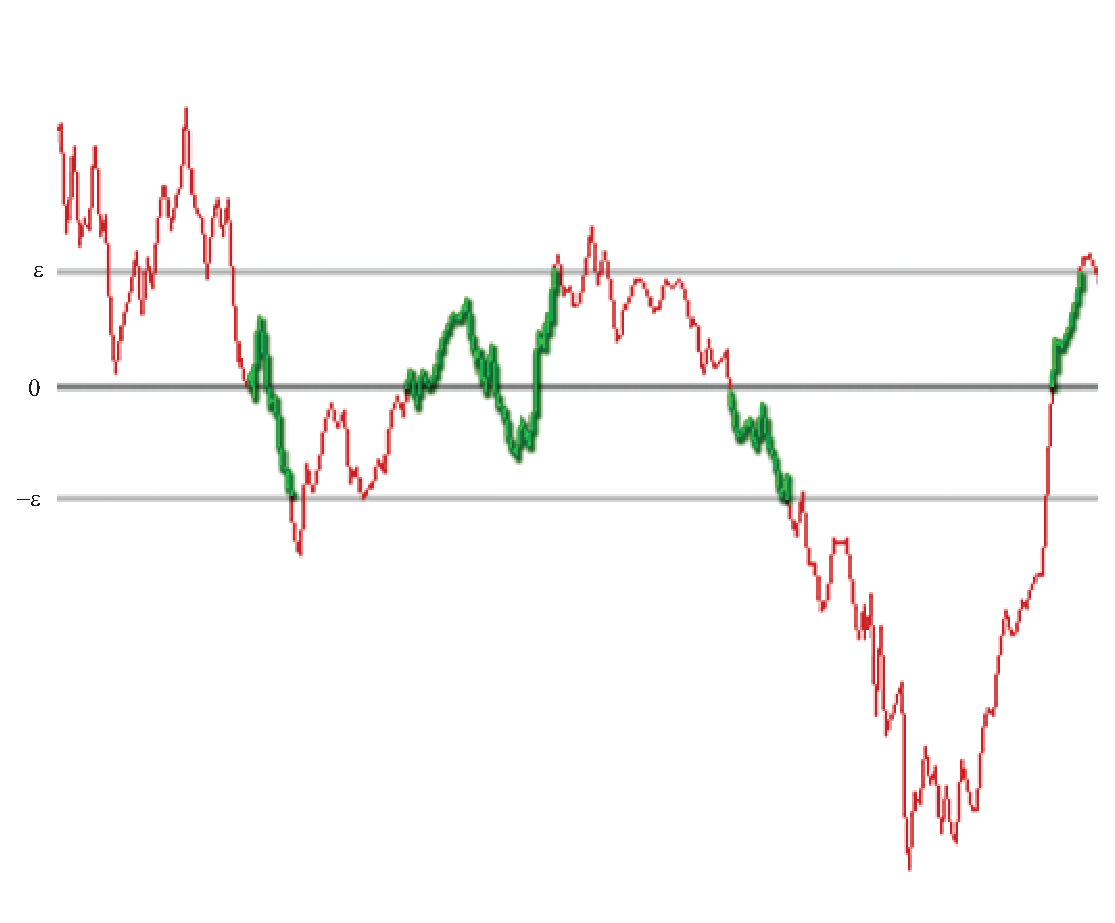
\includegraphics[scale=0.33]{resample1.eps}&
   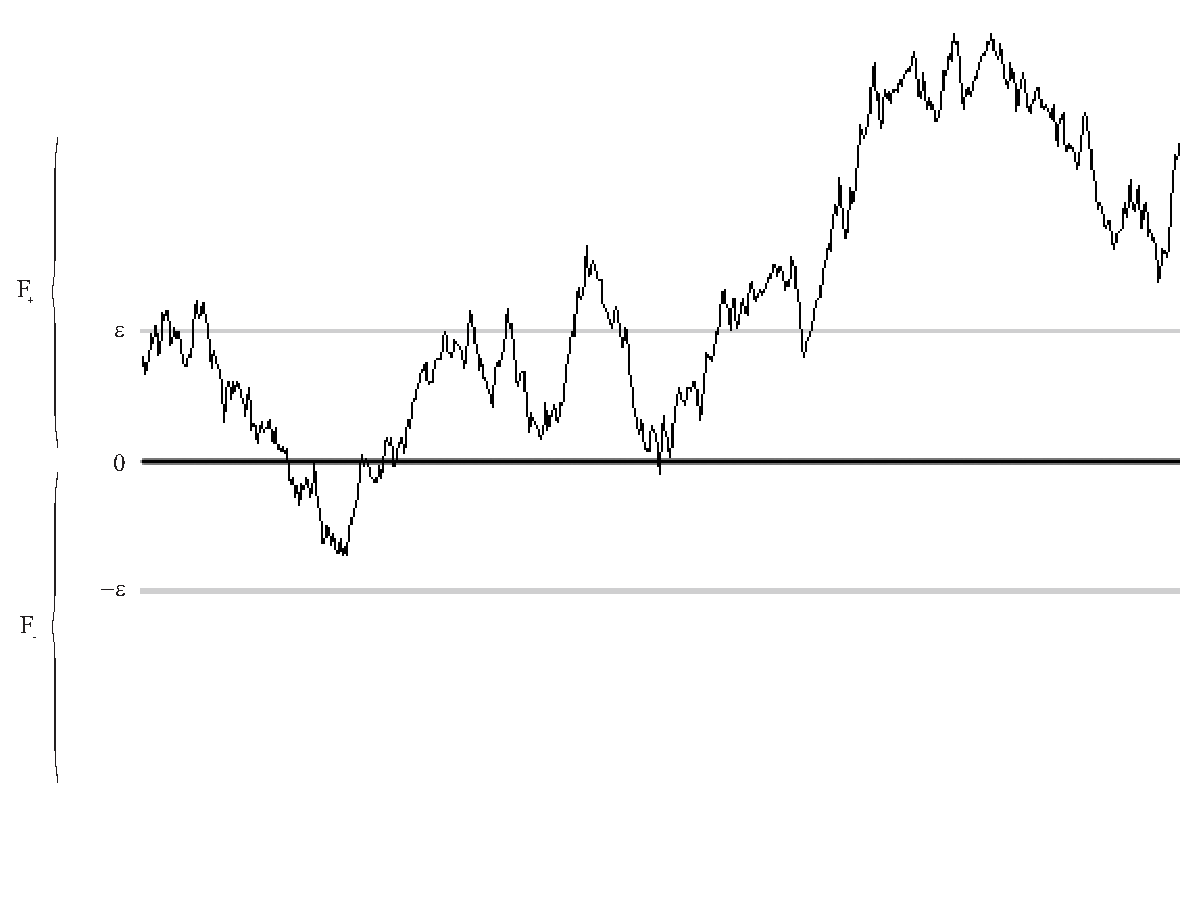
\includegraphics[scale=0.33]{resample2.eps}
   \end{array}$
   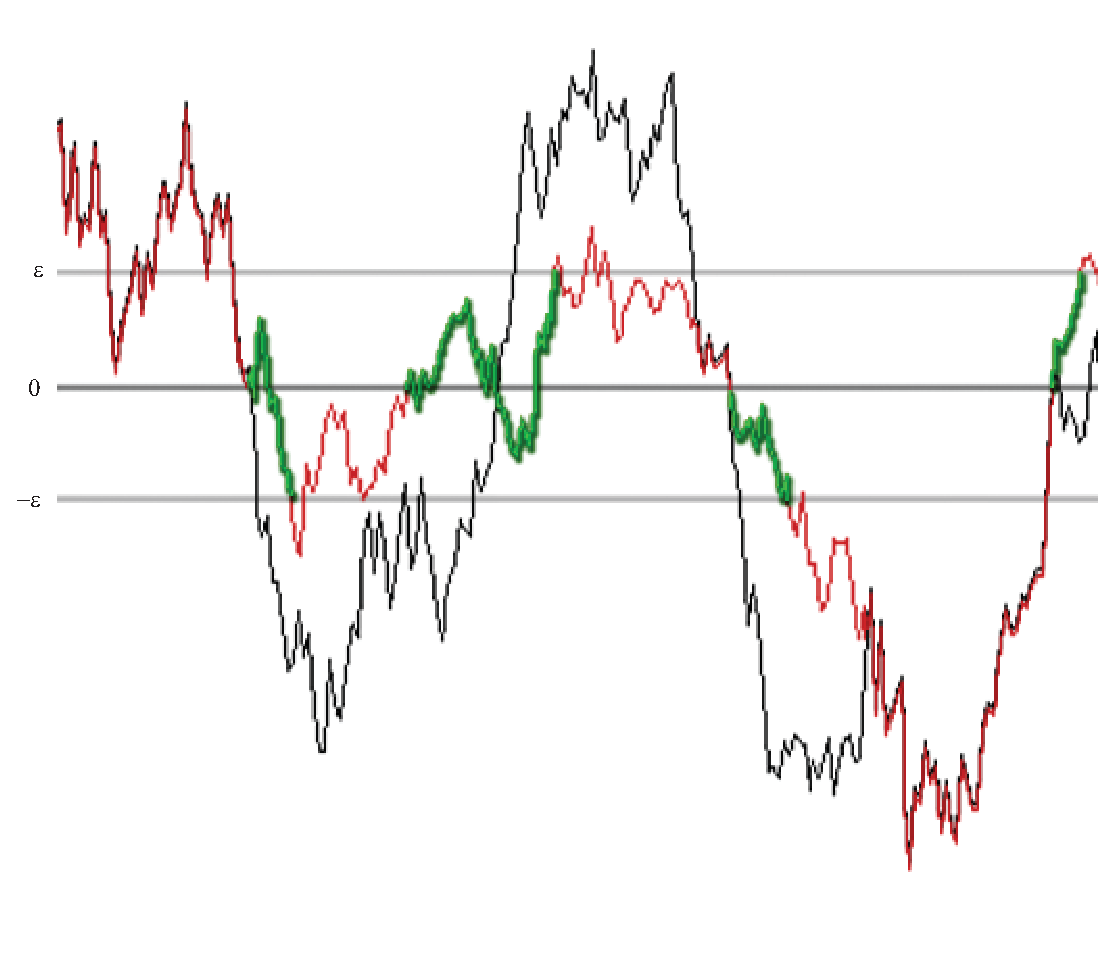
\includegraphics[scale=0.33]{resample.eps}
   \caption{
   A sample of the a web trajectory and the corresponding perturbed processes.
   The top left image depicts the perturbed process, with state B in bold.
   The top right image depicts the original web trajectory. The center image,
   illustrates both processes together, showing the segments where they coalesce.
   }
\end{figure}

The following lemma specifies in what sense the perturbed process is
an approximation of the trajectory of the web.

\begin{lemma}
  \label{lem:resamplede-to-sampled}
  \statementoflemresampledetosampled
\end{lemma}

Lemma \ref{lem:sampled-twostrip-meas} reduces to Lemma
\ref{lem:resamplede-to-sampled}.

\begin{proof}[Proof of reduction]
  $\resamplede$ is $\twostripsreservoir$-measurable, so we use Lemma
  \ref{lem:resamplede-to-sampled} to conclude that $\sampled$ is also
  $\twostripsreservoir$-measurable.  However, since $\sampled$ is
  actually independent of $\reservoir$ we can use a basic result on
  tensor products of Hilbert spaces (for example (1c1), p5 of
  \cite{tsirelson-completion}) to conclude that $\sampled$ is
  in fact $\twostrips$-measurable.
\end{proof}

We devote the following section to the proof of Lemma
\ref{lem:resamplede-to-sampled}.
}

  {
\section{Convergence of the perturbed process}
\label{sec:proof-of-lem:resamplede-to-sampled}

\newcommand{\statenoweb}{S^{2D}_{\indepbm}}
\newcommand{\statewebapart}{S^{2D}_{\webnoargs}}
\newcommand{\statewebtogether}{S^{1D}_{\webnoargs}}
\newcommand{\twodim}{Y}

\newcommand{\twodime}{\twodim(\epsilon)}

In this section we prove that
\statementoflemresampledetosampled{}.  This statement depends only on the
joint distribution of $\sampled$ and $\resamplede$.
We therefore define $\twodime = \twodim=(\resamplede, \sampled)$ (generally suppressing
the $\epsilon$ dependence in the notation). Let us describe the distribution of
$\twodim$
 as a two-dimensional random process.

We classify the behavior of the process into three states according to
the behavior of $\resamplede$ with respect to $\sampled$.
\begin{itemize}
\item If $\resamplede$ is in state $\statewebO$
and is coalesced with $\sampled$ we say $\twodim$ is in
state $\statewebtogether$.
\item If $\resamplede$ is in state $\statewebO$
and \emph{is not} coalesced with $\sampled$ we say $\twodim$ is in state $\statewebapart$.
\item If $\resamplede$ is in state $\statenowebO$
we say $\twodim$ is in state $\statenoweb$.
\end{itemize}
$\twodim$ starts at point $(\startvalue, \startvalue)$ at time $\starttime$
in state $\statewebtogether$.  From $\statewebtogether$, $\twodim$
can only transition to $\statenoweb$.
This transition occurs when $\twodim$ hits the origin, as the coalesced
$\sampled$ and $\resamplede$ will continue together until they leave their
current half-plane.
From $\statenoweb$, $\twodim$ can only transition to
$\statewebapart$.  This transition occurs when $\resamplede$
leaves the $(-\epsilon,\epsilon)$
interval (i.e.\ $\twodim$ hits either of the $x=\pm\epsilon$ lines).
From
$\statewebapart$, $\twodim$ can either transition to $\statewebtogether$
if $\sampled$ and $\resamplede$ coalesce (i.e.\ $\twodim$ hits the line $x=y$)
or transition to $\statenoweb$ if $\resamplede$ hits $0$ (i.e.\ $\twodim$ hits
the $x=0$ line).
States and possible transitions of $\twodim$ are summarized in Figure
\ref{fig:twodimtranstab}.

The form of the labels given to the states is justified by the following.

\begin{observation*}
In $\statewebtogether$, $\twodim$ follows the law of a (time scaled) one-dimensional
Brownian motion on the line $x = y$.
In $\statewebapart$ and $\statenoweb$, $\twodim$ follows the law of a
two-dimensional Brownian motion.
\end{observation*}

Additionally observe that by the scale-invariance of Brownian motion,
the distribution of the sample paths of $\twodime/\epsilon$ is
independent of $\epsilon$ (modulo time scaling).

\begin{figure}
\begin{center}
%  \begin{tabular}{c | l || c | c | c | c | }
\renewcommand{\arraystretch}{0.9}
\begin{tabular}{c|c|c|c|c|c|}
\cline{2-6}
 & State & Illustration & Law & Next & Trans. Cond. \\ \cline{1-6}
\multicolumn{1}{|c|}{\multirow{18}{*}{$\resamplede$}} &
\multicolumn{1}{|c|} {\multirow{6}{*}{$\statewebtogether$}} &  & \multirow{6}{*}{equal} & \multirow{6}{*}{$\statenoweb$} & \multirow{6}{*}{hits $0$}     \\
\multicolumn{1}{|c|} {} & {} & {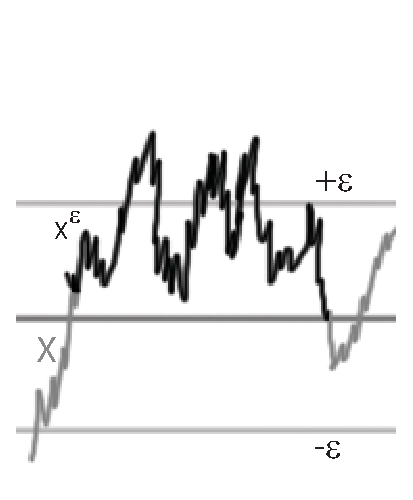
\includegraphics[scale=0.33]{r1d.eps}} & {} & {} &     \\ \cline{2-6}
\multicolumn{1}{|c|} {} &  \multirow{6}{*}{$\statewebapart$} &  & \multirow{6}{*}{indep.} & \multirow{3}{*}{$\statenoweb$} & \multirow{3}{*}{hits   $0$}\\
\multicolumn{1}{|c|} {} & {} & {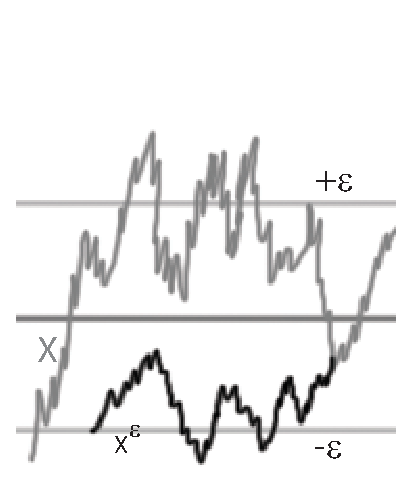
\includegraphics[scale=0.33]{r2dc.eps}} & {} & \multirow{-3}{*}{$\statewebtogether$} &   \multirow{-3}{*}{hits  $\sampled$}  \\ \cline{2-6}
\multicolumn{1}{|c|} {} & {\multirow{6}{*}{$\statenoweb$}} & {}& \multirow{6}{*}{indep.} & \multirow{6}{*}{$\statewebapart$} & \multirow{6}{*}{hits $\pm\epsilon$}     \\
\multicolumn{1}{|c|} {} & {} & {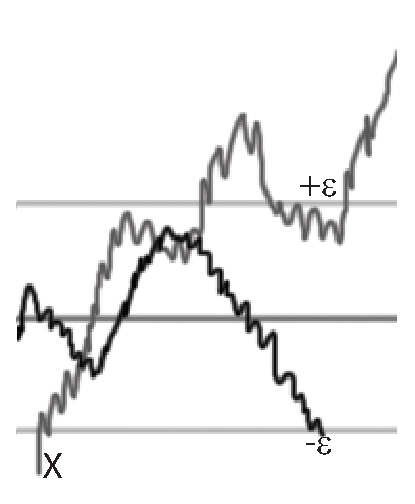
\includegraphics[scale=0.33]{r2dnc.eps}} & {} & {} &      \\ \hline\hline %\cline{1-6}
\multicolumn{1}{|c|}{\multirow{20}{*}{$\twodim=(x,y)$}} &
\multicolumn{1}{|c|} {\multirow{6}{*}{$\statewebtogether$}} &  & \multirow{6}{*}{equal} & \multirow{6}{*}{$\statenoweb$} & \multirow{6}{*}{$x=y=0$}     \\
\multicolumn{1}{|c|} {\multirow{10}{*}{$x=\resamplede$}} & {} & {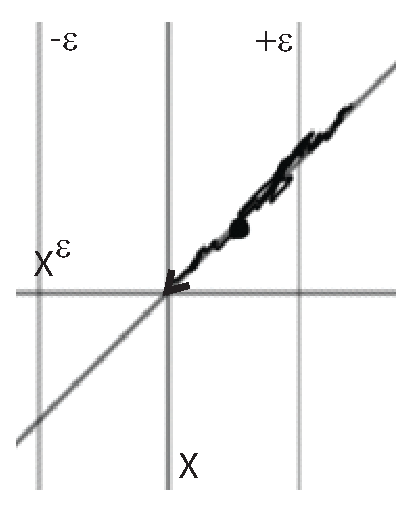
\includegraphics[scale=0.33]{s1d.eps}} & {} & {} &     \\ \cline{2-6}
\multicolumn{1}{|c|} {\multirow{10}{*}{$y=\sampled$}} &  \multirow{6}{*}{$\statewebapart$} &  & \multirow{6}{*}{indep.} & \multirow{3}{*}{$\statenoweb$} & \multirow{3}{*}{$x=0$}\\
\multicolumn{1}{|c|} {} & {} & {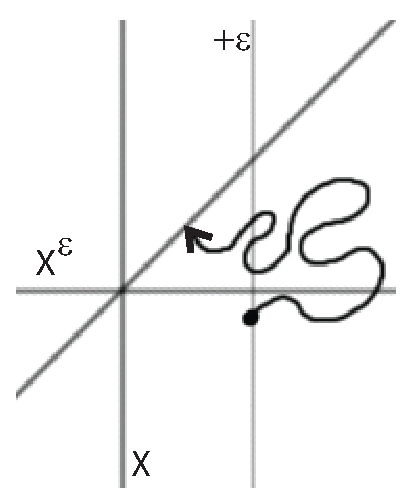
\includegraphics[scale=0.33]{s2dc.eps}} & {} & \multirow{-3}{*}{$\statewebtogether$} &   \multirow{-3}{*}{$x=y$}  \\ \cline{2-6}
\multicolumn{1}{|c|} {} & {\multirow{6}{*}{$\statenoweb$}} & {}& \multirow{6}{*}{indep.} & \multirow{6}{*}{$\statewebapart$} & \multirow{6}{*}{$x=\pm\epsilon$}     \\
\multicolumn{1}{|c|} {} & {} & {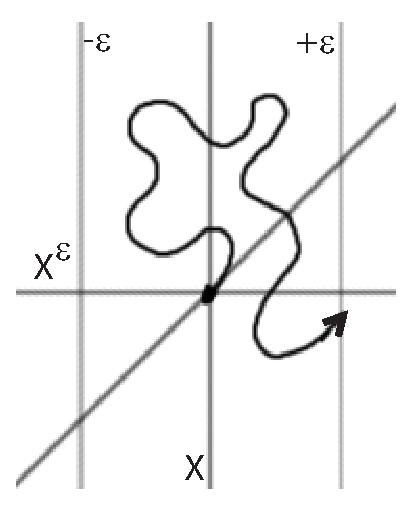
\includegraphics[scale=0.33]{s2dnc.eps}} & {} & {} &    \\
     \hline
  \end{tabular}
\end{center}
\caption{Illustrated states and transitions of $\twodim$}
\label{fig:twodimtranstab}
\end{figure}

\newcommand{\boundarylines}{A_\delta}

Define $\boundarylines=\{(x,y) \ :\  |x-y|=\delta \}$.
To prove Lemma \ref{lem:resamplede-to-sampled} we use the following
property of $\twodim$:

\newcommand{\farpoint}{(P,P)}
\newcommand{\probhitboundaryis}[1]{For given $P > 0$, $\delta > 0$ the probability that $\twodim$
  hits $\boundarylines$ before it hits $\farpoint$ is #1}

\begin{lemma}\label{lem:prob-hit-boundary-o1}
  \probhitboundaryis{$o(1)$ as $\epsilon \to 0$}.
\end{lemma}

Recall that $\twodim$ starts in state $\statewebtogether$, with
$\sampled$ equal to $\resamplede$.  (If $\startvalue = 0$ then $\twodim$
immediately transitions to state $\statenoweb$).
We delay the proof of Lemma \ref{lem:prob-hit-boundary-o1} to Section
\ref{subsec:excursions-of-twodim}.

\begin{proof}[Proof of Lemma \ref{lem:resamplede-to-sampled}]

Lemma \ref{lem:resamplede-to-sampled} is equivalent to: for all $\delta > 0$, $u > \starttime$
\[
\P(\twodim_t \in \{(x,y) \ :\  |x-y|<\delta \} \text{ for all } t \in [\starttime,u])\to1 \text{ as } \epsilon\to 0.
\]
The above statement can be rephrased as

\vspace{12pt}
For all $\delta > 0$, $u > \starttime$,
the probability that before time $u$, $\twodim$ has hit $\boundarylines$
is $o(1)$ as $\epsilon \to 0$.
\DOTHIS{}{Make this display better}
\vspace{12pt}

  We prove this as follows.  For any $\eta > 0$,
  choose $P$ so that the probability that standard Brownian motion
  travels from $0$ to $P$ in time less than $u-\starttime$ is less than
  $\eta$.
  Apply Lemma \ref{lem:prob-hit-boundary-o1} to
  choose $\epsilon_0$ such that, for all $\epsilon < \epsilon_0$, the probability that $\twodime$ hits
  $\boundarylines$ before $\farpoint$ is less than $\eta$.
  Then the probability that $\twodime$ hits $\boundarylines$ before $\farpoint$
  or takes less time than $u-\starttime$ to reach $\farpoint$ is
  less than $2\eta$.
  Thus the probability that $\twodime$ hits $\boundarylines$ before
  time $u$ is less than $2\eta$.
\end{proof}

\subsection{Excursions of $\twodim$}
\label{subsec:excursions-of-twodim}

In this section we prove the following, which is slightly stronger than
Lemma \ref{lem:prob-hit-boundary-o1}.

\newcommand{\loger}{\log 1/\epsilon}

\begin{lemma}\label{lem:prob-hit-boundary-o1loge}
  \probhitboundaryis{$O(\frac{1}{\loger})$}.
\end{lemma}

\newcommand{\origin}{(0,0)}

\newcommand{\excursionstart}{T}
\newcommand{\hitset}{U}
\newcommand{\hitevent}[1]{H_{#1}}
\newcommand{\hiteventi}{\hitevent{i}}

The random set $\{t \ge \starttime : \twodim_t = \origin\}$ is almost surely
infinite and discrete. We can therefore order this set, writing $T_0$
for its smallest element, $T_1$ for the next, and so on.

Let $\hitset \subset \R^2$ and write $\hiteventi$ for the event
$\{\twodim_t \in \hitset \text{ for some } t \in
[T_i,T_{i+1}]\}$. Observe that since our process starts and ends every
time interval of the form $[T_i,T_{i+1}]$ at $\origin$ (and in state
$S_\psi^{2D}$) the events $\{\hiteventi : i \ge 0\}$ are independent
and have the same probability.  We call this probability ``the
probability that an excursion hits a set $U$''.
  \TODO{}{Provide a justification for the well-definedness of these
    stopping times, perhaps in terms of the states?}

\newcommand{\probexcursionhits}[1]{\P\left(\text{an excursion hits } #1\right)}

Our approach to proving Lemma \ref{lem:prob-hit-boundary-o1loge} is to
demonstrate that
\[
\probexcursionhits{\farpoint} \gg
\probexcursionhits{\boundarylines} \text { as } \epsilon \to 0.
\]
This is
realized through the next pair of lemmas whose proofs we delay until Section
\ref{proofs-of-the-excursion-lemmas}.

\newcommand{\Omegaeloge}{\Omega(\epsilon\loger)}

\begin{lemma}
  \label{lem:Phitboundaryline}
  For given $\delta > 0$, $\probexcursionhits{\boundarylines}$ is $O(\epsilon)$.
\end{lemma}

\begin{lemma}
  \label{lem:Pabsorbedandtravelsfar}
  For given $P > 0$, $\probexcursionhits{\farpoint}$ is $\Omegaeloge$.
\end{lemma}

\newcommand{\Oe}{O(\epsilon)}

\begin{proof}[Proof of Lemma \ref{lem:prob-hit-boundary-o1loge}]
  $\twodim$ consists of a sequence of excursions, each of which satisfies
  exactly one of the following conditions
  \begin{itemize}
  \item the excursion hits $\boundarylines$ (with probability
    $O(\epsilon$)),
  \item the excursion does not hit $\boundarylines$ but does hit
    $\farpoint$ (with probability $\Omegaeloge-\Oe$, which is itself
    $\Omegaeloge$),
  \item the excursion does not hit $\boundarylines$ or $\farpoint$.
  \end{itemize}
  The excursions are independent, so the probability that $\twodim$
  hits $\boundarylines$ before $\farpoint$ is
  \[
  \frac{\Oe}{\Omegaeloge + \Oe} = O\left(\frac{1}{\loger}\right).
  \]
\end{proof}

\subsection{Proofs of the excursion lemmas}
\label{proofs-of-the-excursion-lemmas}
\newcommand{\tdh}{\rotproc^1}
\newcommand{\tdv}{\rotproc^2}
\newcommand{\rotproc}{Z}

\DOTHIS{}{Perhaps should introduce more consistency between $\rotproc$
  and $\twodim$ in this proof}
{
\newcommand{\x}{\resamplede}
\newcommand{\y}{\sampled}
In this section we give the proof of Lemmas \ref{lem:Phitboundaryline} and
\ref{lem:Pabsorbedandtravelsfar}. For convenience we rotate (and scale)
$\twodim=(\x,\y)$, defining
\[\rotproc(\epsilon) = \rotproc=(\tdh,\tdv)=\frac{1}{2}(\x+\y,\x-\y).\]

Observe that when $\twodim$ is in $\statewebtogether$, $\rotproc$ follows
the law of a standard one-dimensional Brownian motion on the $x$-axis.
The condition that $\twodim$ hits $\boundarylines$ is equivalent
to $\tdv$ hitting $\pm\delta/2$.
Like $\twodim$, $\rotproc$ has the following ``scale invariance''
property: the distribution of sample paths of $\rotproc(\epsilon) /
\epsilon$ is independent of $\epsilon$ (modulo time scaling).

\begin{proof}[Proof of Lemma \ref{lem:Phitboundaryline}]
Consider the process $\twodim$ between times $\excursionstart_0$ and
$\excursionstart_1$.  Once $\twodim$ arrives at $\statewebtogether$ it
can never hit $\boundarylines$ before hitting $\origin$.  Thus our
goal is to show that with probability at least $1-O(\epsilon)$,
$\twodim$ arrives in $\statewebtogether$ before hitting
$\boundarylines$.  Next, we observe the
following two auxiliary claims:

\begin{claim}\label{cl:tdv-together-estimate}
  Whenever $\tdv=0$ the probability that subsequently $\twodim$
  arrives at $\statewebtogether$ before $\tdv$ hits $\pm\epsilon/2$ is
  at least a constant (independent of $\epsilon$).
\end{claim}

\begin{claim}\label{cl:tdv-hitting-back-0-estimate}
  Whenever $\tdv=\pm\epsilon/2$ then there is probability equal to
  $\epsilon/\delta$ of $\tdv$ hitting $\pm\delta/2$ before it hits $0$.
\end{claim}

Claim \ref{cl:tdv-together-estimate} follows from scale invariance, while
Claim \ref{cl:tdv-hitting-back-0-estimate} is a standard martingale result on
Brownian motion (observing that on the relevant time interval $\tdv$ is a
standard Brownian motion).

The reduction of Lemma \ref{lem:Phitboundaryline} to those two claims is
similar to the proof of Lemma \ref{lem:prob-hit-boundary-o1loge}. Claims
\ref{cl:tdv-together-estimate} and \ref{cl:tdv-hitting-back-0-estimate} imply
that between a time when $\tdv = 0$ and the next time that
$\tdv = 0$ after having hit $\pm\epsilon/2$,
\[
\frac{\P(\twodim\text{ hits }\boundarylines)}{\P(\twodim\text{arrives at }\statewebtogether)}
\le \frac{(1-C)(\epsilon/\delta)}{C} =O(\epsilon)
\]
\DOTHIS{}{these probabilities are a bit confusing}
where $C$ is the constant of Claim \ref{cl:tdv-together-estimate}. As the
behavior of $\twodim$ is independent on those intervals, we deduce Lemma
\ref{lem:Phitboundaryline}.

\DOTHIS{}{Why did we need independence?}
\end{proof}
}
\begin{proof}[Proof of Lemma \ref{lem:Pabsorbedandtravelsfar}]
\newcommand{\rotfarpoint}{(P,0)}
\newcommand{\segment}{[\epsilon,1] \cross \{0\}}
We bound below the probability that an excursion hits $\farpoint$,
i.e.\ $\rotproc$ hits $\rotfarpoint$ before returning to $\origin$.
We do this by considering the probability that the excursion takes
the following form: $\rotproc$ travels from $\origin$ to the line
segment $Q = [0, \epsilon] \cross \{\epsilon\}$, then hits the horizontal
axis for the first time in $\segment$, then travels to $\rotfarpoint$,
before returning to $\origin$.

After a stopping time at which $\twodim = \rotproc = \origin$ there is a positive probability $K$
that $\rotproc$ hits $Q$ before returning to $\origin$.
By scale invariance $K$ is independent of $\epsilon$.

Consider $\rotproc$ after hitting some point in $Q$.  We now
bound the hitting density of this process on the horizontal
axis.  Regardless of the point in $Q$, this density for points on
$\segment$ is at least
\[
\frac{1}{\pi\epsilon} \frac{1}{1 + (x/\epsilon)^2} dx.
\]
This follows directly from the classical result that the hitting density
on a line of the two-dimensional Brownian motion is a Cauchy distribution
(see for example Theorem 2.37 of \cite{mortens-peres}).

On hitting a point $(x,0)$ for $x \in [\epsilon, 1]$ the process
transitions from state $\statewebapart$ to state $\statewebtogether$.
When in state $\statewebtogether$, $\rotproc$ behaves as a
one-dimensional Brownian motion on the horizontal axis until it hits
$\origin$.
By the same martingale argument which justifies
Claim \ref{cl:tdv-hitting-back-0-estimate}, the
probability of subsequently hitting $\rotfarpoint$ before $\origin$ is $x/P$.
Integrating this against the hitting density we get that the probability that
$\rotproc$ started from some point in $Q$ hits the horizontal axis in $\segment$
and then travels to $\rotfarpoint$ before returning
to $\origin$ is at least
\[
\frac{1}{\pi P} \int_{\epsilon}^{1} \frac{x/\epsilon}{1 + (x/\epsilon)^2}
\, dx
=
\frac{\epsilon}{2\pi P} \log\left(\frac{1 + (1/\epsilon)^2}{2}\right)
,\text{ which is }
\Omegaeloge.
\]
\TODO{}{This now looks slightly odd}
\end{proof}
}

  {
\section{Recovering the Brownian web from its strips}

We will define a $\sigma$-algebra $\factor{y}{z}$ for each $y < z \in
[-\infty, \infty]$ which corresponds to the information contained in
the trajectories of the Brownian web in the horizontal strip
$(-\infty, \infty) \cross (y,z)$.

\begin{definition}
  \newcommand{\T}{\stripleavetime{f}}
  \label{def:restrict}
  From a path $f : [s, \infty) \to \R$ we define ``$f$ stopped on
    leaving the interval $(a,b)$'' to be the map $\restrict{a}{b}{f} : [s,
      \infty) \to \R$ given by $\restrict{a}{b}{f}(t) = f(t \minsym \T)$
      where $\T = \inf\{ t : f(t) \not\in (a,b) \}$.
\end{definition}

\TODO{}{Note that the path $f$ may start outside the strip, in which
  case we consider it stopped immediately.}

\newcommand{\brownianwebnoise}{collection of horiztontal
  sub-$\sigma$-algebras of the Brownian web}

\begin{definition}
  The \brownianwebnoise{} is an
  association of a $\sigma$-algebra $\factor{y}{z}$ to each $(y, z)
  \in \simplex$, generated by the following collection of paths:
  $\{ \restrict{y}{z}{t \mapsto \web{s}{t}{x}} : s, x \in \R \}$
\end{definition}

With these definitions, $\upperhp$ of Section \ref{recovering-from-half-planes} is
$\commafactor{0}{\infty}$ and $\lowerhp$ is
$\commafactor{-\infty}{0}$.

\begin{observation}
  Note that $\factor{w}{x}$ and $\factor{y}{z}$ are independent if the
  intervals $(w,x)$ and $(y,z)$ are disjoint.
\end{observation}

\renewcommand{\top}{b}
\newcommand{\bottom}{a}

For notational convenience in the rest of this
section we will fix $\bottom < 0 < \top$ and write $\Res{\cdot}$ for
$\restrict{\bottom}{\top}{\cdot}$.

\newcommand{\Resresamplede}{\Res{\resamplede}}
\newcommand{\Ressampled}{\Res{\sampled}}

The collection of variables of the form $\Ressampled$ generates
$\factor{\bottom}{\top}$, and the aim is to show that in fact each $\Ressampled$ can
be recovered from information in $\factor{\bottom}{0}$ and $\factor{0}{\top}$
only.

Note that $\Resresamplede$ is what you obtain when you perform the
procedure of Definition \ref{def:resamplede} on paths in the
$(\bottom,0)$-strip and the $(0,\top)$-strip, rather than the upper and lower
half-planes.  The $\reservoir$-measurable Brownian motion is still used to
cross the gap between the strips, which is at level $0$.

Like in Section \ref{recovering-from-half-planes}, $\Resresamplede$
is constructed from information in $\factor{\bottom}{0}$,
$\factor{0}{\top}$ and $\reservoir$ only.

\begin{observation}
  $\Res{\resamplede}$ is $\factor{\bottom}{0} \tensor \factor{0}{\top}
  \tensor \reservoir$-measurable.
\end{observation}

Furthermore, we will show that as $\epsilon \to 0$ we have that
$\Resresamplede$ approaches $\Ressampled$.  We could show this
directly by an extension of the argument we used for the half-planes
in Section \ref{recovering-from-half-planes}.  However, knowing that
$\resamplede \toinP \sampled$ is nearly enough, and all that is required
in addition is to show that this convergence is preserved by the
restriction map $\Res{\cdot}$.

To show that the convergence is preserved we use the following
property of the restriction map.

\newcommand{\stripleavetimenotturningpoint}[1]{$\stripleavetime{#1}$ is
  not a turning point of the path $#1$}

\begin{lemma}
  \label{lem:Res-continuous-ae}
  If \stripleavetimenotturningpoint{f},
  then the map $f \mapsto \Res{f}$ is continuous at $f$ in the
  topology of uniform convergence on compacts.
\end{lemma}

\begin{proof}
  \DOTHIS{We sketch a proof of this straightforward result in
    classical analysis.

    \newcommand{\fn}{f_n}

    \newcommand{\T}{\stripleavetime{f}}
    \newcommand{\Tn}{\stripleavetime{\fn}}
    \newcommand{\starttime}{s}

    Suppose $\fn \to f$ uniformly on compacts, and both are paths
    starting at time $\starttime$

    If $\T = \infty$ there is very little to prove, so suppose
    otherwise.  Then since $\T$ is not
    a turning point of $f$ it is easily seen that $\Tn \to \T$ and
    that eventually \DOTHIS{$\fn(\Tn) = f(\T)$}{They both take the value
      either $\bottom$ or $\top$ -- or both of them start outside the
      strip}.

    \renewcommand{\d}{\delta}
    \newcommand{\e}{\epsilon}

    Since $f$ is continuous, choose $\d$ such that
    $|f(\T) - f(x)| \le \epsilon$ when
    $|\T - x| \le \delta$.  Eventually
    \begin{itemize}
    \item $\fn(\Tn) = f(\T)$
    \item $|\Tn - \T| \le \d$
    \item $|\fn - f| \le \e$ uniformly on some compact containing
      $[\starttime, \T+\d]$.
    \end{itemize}

    \newcommand{\stoppedfn}{\Res{\fn}}
    \newcommand{\stoppedf}{\Res{f}}

    \newcommand{\condition}[2]{for $t \in {#1}$ we have
      $|\stoppedfn(t) - \stoppedf(t)| #2$}
    so
    \begin{itemize}
    \item \condition{[\starttime, \T-\d)}{\le \e}
    \item \condition{[\T-\d, \T+\d]}{\le 2\e}
    \item \condition{(\T+\d, \infty)}{= 0}
    \end{itemize}
    so indeed $\stoppedfn \to \stoppedf$ uniformly on compacts.}
      {The only tricky part is the second item.  There are
      four cases to consider.  The worst case is when $\stoppedf$ has
      been truncated and $\stoppedfn$ hasn't.  But $\stoppedf$ is
      equal to the level, and so is within $\e$ of $f$.  OTOH
      $\stoppedfn = \fn$ so is within $\e$ of $f$.  Thus the $2\e$
      bound.}
\end{proof}

Observe that sample paths of Brownian motion $\sampled$ almost surely
satisfy the condition of the lemma, that
``\stripleavetimenotturningpoint{\sampled}''.  This allows us to reach
the desired convergence result.

\begin{lemma}
  $\Res{\resamplede} \toinP \Res{\sampled}$ as $\epsilon \to 0$
\end{lemma}

\begin{proof}
  We already know that $\resamplede \toinP \sampled$, and in addition
  the probability that $f \mapsto \Res{f}$ is continuous at $X$ is $1$
  (by Lemma \ref{lem:Res-continuous-ae}).
  So we conclude that $\Res{\resamplede} \toinP
  \Res{\sampled}$ by the continuous mapping theorem (see for
  example \cite{billingsley}, p. 21, Theorem 2.7).
\end{proof}

As in Section \ref{recovering-from-half-planes} we can conclude that

\begin{lemma}
  $\Res{\sampled}$ is $\factor{\bottom}{0} \tensor
  \factor{0}{\top}$-measurable.
\end{lemma}

\subsection{What does this mean in terms of noises?}

As before we can conclude that

\begin{theorem}
  $\factor{\bottom}{\top} = \factor{\bottom}{0} \tensor \factor{0}{\top}$
\end{theorem}

There was nothing special about the split between the strips being at
level $0$, so in fact we have shown that

\begin{cor}
  $\factor{x}{z} = \factor{x}{y} \tensor \factor{y}{z}$ for all $x < y < z$
\end{cor}

\begin{theorem}
  The \brownianwebnoise{}
  is a continuous product of probability spaces in the sense that
  for each $x \le y \le z$, $\factor{x}{y} \tensor \factor{y}{z} =
  \factor{x}{z}$.
  See 3c1 Definition of
  \cite{tsirelson-nonclassical-stochastic-flows}.
\end{theorem}

\begin{theorem}
  The \brownianwebnoise{} is a noise in the sense that it is a
  continuous product of probability spaces with a translation.
  See 3d1 Definition of
  \cite{tsirelson-nonclassical-stochastic-flows}.
\end{theorem}

\FIXME{}{Need to make a comment that the obvious translation works.}

\begin{theorem}
  The collection of two-dimensional sub-$\sigma$-algebras of the
  Brownian web is a two-dimensional noise, and moreover it is black.
\end{theorem}

\begin{proof}
  We know that the one-dimensional noise consisting of the vertical
  collection of sub-$\sigma$-algebras is black.  By general arguments
  on spectral sets this implies that the two-dimensional noise is
  black.  See \cite{tsirelson-classicality-blackness-spectrum}.
\end{proof}

}

%  {
\newcommand{\eeps}{e_\epsilon}

\section{Suitable title}
Let $(x, \eeps)$ be a pair with distribution the same as the two
dimensional process from Observation \ref{obs:2d-proc}.

Our goal in this section is to prove the following theorem:
\begin{theorem}\label{thm:main1}
Under the previous notations, $\eeps(1) \to x(1)$ in probability
as $\epsilon \to 0$.
\end{theorem}

\newcommand{\radiussq}{\delta^2}
\newcommand{\radius}{\delta}
\newcommand{\twonorm}[1]{||#1||_2}

\newcommand{\twodproc}[1]{(x(#1), \eeps(#1))}

In order to prove this it will be easier to prove the following
stronger claim:
\begin{propos}\label{thm:main2}
For every $t\in[0,1]$ and every $\radius>0$
$$\ds \lim_{\epsilon \rightarrow 0}\P\left(\text{either } x(t)=\eeps(t)
\text{ or } \twonorm{\twodproc{t}} <\radius\right)=1$$
Equivalently, until time $1$, the two dimensional process $\twodproc{t}$
leaves the $\radius$ disc only through $(\frac{\radius}{\sqrt2},\frac{\radius}{\sqrt2})$ or through $-(\frac{\radius}{\sqrt2},\frac{\radius}{\sqrt2})$, with high probability.
\FIXME{}{I'm not completely comfortable with this equivalent
  definition.  It's informal, though it has a formal counterpart, and
  it doesn't seem immediate that the formal counterpart is equivalent
  to Proposition \ref{thm:main2} -- Tom}
\end{propos}

We begin by presenting a handy property whose proof
we delay to Subsection \ref{sec:POC}:

\begin{propos}\label{thm:no-escape}
Suppose that at time $t_0$ we have
$\twodproc{t_0}=(0,0)$, let $t>0$ be the first time at which
$\twonorm{\twodproc{t}}=1$, then the probability
that $\twodproc{t} \not=\pm(\frac{1}{\sqrt2},\frac{1}{\sqrt2})$ is $O(\frac1{\log\epsilon})$.
\end{propos}

Applying scaling invariance to this theorem immediately yields the
following corollary:
\begin{cor}\label{cor:cor1}
Let $\radius>0$ suppose that at time $t_0$ we have $\twodproc{t_0}=(0,0)$, let
$t>0$ be the first time at which
$\twonorm{\twodproc{t}} = \radius$, then the probability
that $\twodproc{t} \not=\pm(\frac{\radius}{\sqrt2},\frac{\radius}{\sqrt2})$ is
$O(\frac{1}{\log\epsilon/\radiussq})$.
\end{cor}

In order to overcome the gap between Corollary \ref{cor:cor1} and
Theorem \ref{thm:main1} we quote without proof the following property of Brownian
motion:
\begin{propos}\label{prop:prop1}
Let $\zeta>0$ and let $x(t)$ be a one dimensional Brownian
motion such that $x(0)=0$. There exist some $k$ such that
$\P(\ds\sup_{t\in[0,1]}x(t)>k) <\zeta$.
\end{propos}

We are now ready to give a proof to Proposition \ref{thm:main2}.

\begin{proof}[Proof (Proposition \ref{thm:main2})]
\newcommand{\hitradius}[1]{\twonorm{\twodproc{#1}}=\radius}

Let us think of $b(t)=\twodproc{t}$ as a process which dies if ever $x(t)\neq\eeps(t)
\text{ or } \twonorm{\twodproc{t}} = \radius$.

We define a one-dimensional "$\radius$-Teleporting" Brownian motion: $x^{\radius}(t)$
 as a Brownian motion such that whenever it hits $0$ it teleports to $\frac1{\sqrt{2}}\radius$.
Proposition \ref{prop:prop1} implies that for all $\zeta>0$ there exists a $k$ such that the probability
that $x^{\radius}(t)$ is teleported more then $k$ times between times $0$ and $1$ is less then $\zeta$. Let $x^{\radius}(t)$ be such a teleporting Brownian motion, and let
 $d_i(t)=\twodproc{t}_i$ be an infinite sequence
 of independent random walks identical in distribution to $b(t)$, starting from $(0,0)$, such that each
 of them dies when $\twonorm{\twodproc{t}} = \radius$. We can now couple $b(t)$ with the set $\{x^\radius(t)\}\ds\bigcup_{i=1}^\infty\{d_i(t)\}$ in the following way:

Set $t_0=0$. We begin by coupling $d_1(t)$ with $b(t)$ until $d_1(t)$ terminates at 
time $t'_0$, if $x(t'_0)\neq\eeps(t'_0)$ then $b(t)$ terminates as well, otherwise
 if $x(t_0)=\frac1{\sqrt{2}}\radius$ we couple $b(t)$ with $(\frac{x^\radius(t-t'_0+t_0)}{\sqrt{2}},\frac{x^\radius(t-t'_0+t_0)}{\sqrt{2}})$,
  and if $x(t_0)=-\radius$ we couple $b(t)$ with $-(\frac{x^\radius(t-t'_0+t_0)}{\sqrt{2}},\frac{x^\radius(t-t'_0+t_0)}{\sqrt{2}})$.
 This continues until time $t_1$, the first to satisfy $b(t_1)=(0,0)$ after $t'_0$, 
 at which we couple $b(t)$ with $d_2(t-t_1)$, and so on and so forth.

Let us look at the event that $x^\radius(t)$ has teleported at most $k$ times by time $1$.
 By Proposition \ref{prop:prop1} we can pick $k$ such that this probability will be as small 
 as we want. The events that $d_i$ for $i\le k$ terminated on a point such that $x=\eeps$ 
 are independent and by Corollary \ref{cor:cor1} can be made as small as we want. However
  if both events do not occur - the coupling insures us that by time $t=1$ the two
   dimensional process $b(t)$
leaves the $\radius$ disc only through
$\frac1{\sqrt2}(\radius,\radius)$ or through
$\frac1{\sqrt2}(-\radius,-\radius)$. We deduce that the two dimensional process $b(t)=\twodproc{t}$
a.s.\ leaves the $\radius$ disc only through $(\frac{\radius}{\sqrt2},\frac{\radius}{\sqrt2})$ or through $-(\frac{\radius}{\sqrt2},\frac{\radius}{\sqrt2})$.

\end{proof}

\subsection{Proof of convergence}\label{sec:POC}
{
%Let $\xi_\epsilon=(X,Y,\epsilon)$ as before. We denoted by $\eeps(t)$ a sample of $\xi_\epsilon$
%starting at some given point at time $0$. We also denote by $x(t)$ a
%sample of $X$ starting at the same point.
%NB: \xi no longer exists above -- Tom
In this section we prove Proposition \ref{thm:no-escape}. Our main technical tool in doing so will
be conformal maps. We begin by rotating the process $\twodproc{\cdot}$
through $\pi/4$ radians clockwise about the origin to get a process
$b_\epsilon(t)$ \FIXME{which is absorbing only along the \FIXME{$x$
    axis}{$x$ is a constant in earlier notation}}{this is a note to
  make it clearer to the reader exactly what's going on, but perhaps
  it should be clearer}.
Sometimes, we will omit the $\epsilon$ writing $b(t)$. \FIXME{We always assume $\epsilon$
to be sufficiently small.}{This is a confusing statement.  What does
  it actually mean?  Are there actually any cases where this
  assumption is used?  If not, let's delete it -- Tom}
We can now rephrase Proposition
\ref{thm:no-escape} as:

\begin{propos}[Proposition \ref{thm:no-escape} rephrased]\label{prop:reph}
Suppose that at time $t_0$ we have
${b}(t_0)=(0,0)$, let $t_1>0$ be the first time at which
$||b(t_1)||_2=1$, then the probability that $b(t_1)\neq \pm(1,0)$ is
$O\left(\frac1{\log\epsilon}\right)$.
\end{propos}

We define the following indicator function
\newcommand{\online}[1]{A(#1)}
\[\online{t} := (b(t) \text{ is on the x axis and its x component has modulus
} > \epsilon)\]
Note that whenever $\online{t}=1$,
we can regard $b(t)$ as a one dimensional Brownian motion on the
$x$-axis, while whenever $\online{t}=0$ we can regard it as a two
dimensional Brownian motion. We can now treat the sampled
process $b_\epsilon(t)$ as a state machine with $4$ states
$a_0,a^r_1,a_{\text{win}},a_{\text{lose}}$, one of which ($a^r_1$) has a parameter $r$.

The states are defined in the following way:
\begin{enumerate}
\item\label{n1} $b_\epsilon(t)$ is in state $a_0$ whenever $\online{t}=0$.
\item\label{n2} $b_\epsilon(t)$ is in state $a^r_1$ whenever
  $\online{t}=1$ and \FIXME{$|x(\sup_{s<t}(\online{s}=0))|=r$}{this is
  not right}.
\item\label{n3} $b_\epsilon(t)$ is in state $a_\text{win}$ whenever $b_\epsilon(t)=\pm(1,0)$.
\item\label{n4} $b_\epsilon(t)$ is in state $a_\text{lose}$ whenever $b_\epsilon(t)\neq\pm(1,0)$ yet $||b_\epsilon(t)||_2=1$.
\end{enumerate}

By this definition, at time $0$ our state machine is in state $a_0$.
We strive to prove that the probability to get to
 state $a_\text{lose}$ before getting to $a_\text{win}$ is $O(\frac1{\log\epsilon})$.
 We do this by calculating the transition functions of
 this state machine. This calculation is describe by the following proposition,
 while the state machine is depicted in Figure \ref{fig:state_machine}.

 \begin{figure}[htb]
\begin{center}
\leavevmode
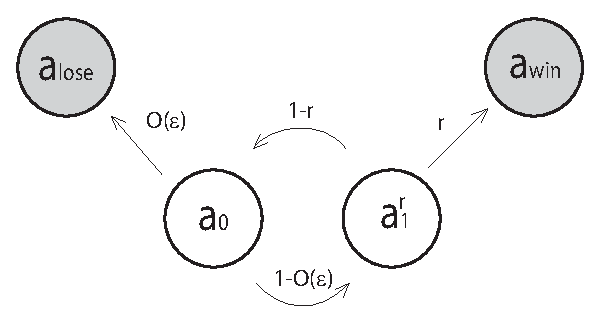
\includegraphics{state_machine.eps}
\end{center}
\caption{A diagram of the state machine.}
\label{fig:state_machine}
\end{figure}

\begin{propos}[Transition probabilities]\label{prop:trans}
The following is the transition probability of the state machine described above:
\begin{enumerate}
\item\label{m11} $\P(a^r_1\rightarrow a_0)=1-r$
\item\label{m12} $\P(a^r_1\rightarrow a_\text{win})=r$
\item\label{m13} $\P(a^r_1\rightarrow a_\text{lose})=0$
\item\label{m21} $\P(a_0\rightarrow a_\text{win})=0$
\item\label{m22} $\P(a_0\rightarrow a_\text{lose})=O(\epsilon)$
\item\label{m23} $\P(a_0\rightarrow a^r_1 \text{ for some }r)=1-O(\epsilon)$
\item\label{m24} $\P(a_0\rightarrow a^r_1 \text{ such that } r_0<r<r_1)>\ds c\epsilon\left(\frac 1 {r_0}-\frac 1 {r_1}-1\right)$ for $r_0>2\epsilon$.
%$\P(a_0\rightarrow a^r_1 \text{ such that } r_0<r<r_1)>\ds\int_{r_0}^{r_1}(\frac{c\epsilon}{r^2}-0.5)dr$ for $r_0>2\epsilon$
\end{enumerate}
$a_\text{win}$ and $a_\text{lose}$ are trap states which are assigned no transition function.
\end{propos}

\begin{proof}
 On $a^r_1$ we know $b(t)$ is a $1$-dimensional Brownian motion starting at $r$.
 We can treat the transition time of $b(t)$ from $a^r_1$ to either $a_0$ or
 $a_\text{win}$ as a stopping time for such a Browinian motion, getting
 \ref{m11} and \ref{m12} immediately. The definition of the different states
 implies \ref{m13} and \ref{m21}. The proofs of \ref{m22}, \ref{m23} and \ref{m24}
 are given separately in Corollaries \ref{m22and23true} and \ref{m24true} in Section \ref{sec:ROI}.
\end{proof}

Analyzing the transition probabilities described in Proposition \ref{prop:trans} we
can find the probability of reaching $a_\text{lose}$ before $a_\text{win}$ and vice versa.
 The main step towards this result is the following proposition:

\begin{propos}\label{prop:winlose1}
Let $s_1=a_0,...,s_n$ be the sequence of states of our state machine.
\begin{equation}\label{eq:losecase}
\P(s_n=a_\text{lose} \text{ and } \ds\forall_{i>1}(s_i\neq a_0))=O(\epsilon)
\end{equation}
\begin{equation}\label{eq:wincase}
\P(s_n=a_\text{win} \text{ and } \ds\forall_{i>1}(s_i\neq a_0))=\Omega(\epsilon\log\epsilon)
\end{equation}
\end{propos}

\begin{proof}
Both \eqref{eq:losecase} and \eqref{eq:wincase} are direct results of Proposition \ref{prop:trans}.
 $a_0$ can be followed only by $a_\text{lose}$ and $a_1^r$. However $a_\text{lose}$ cannot be
 reached from $a_1^r$ without passing through
 $a_\text{win}$, thus:
 $$\P(s_n=a_\text{lose} \text{ and } \ds\forall_{i>1}(s_i\neq a_0))=\P(a_0\rightarrow a_\text{lose})=O(\epsilon)$$
 where the last equality is by item \ref{m22} in Proposition \ref{prop:trans}.
 This concludes the proof of \eqref{eq:losecase}.

 In order to reach $a_\text{win}$ from $a_0$, we must have $a_1^r$ following $a_0$, and then $a_\text{win}$
  following $a_1^r$. By Fubini's Theorem, this yields the following formula:
 \begin{equation}\label{eq:r1}
 \P(s_n=a_\text{win} \text{ and } \ds\forall_{i>1}(s_i\neq a_0))=\ds\int_{\epsilon}^1 f(r) \P(a^r_1\rightarrow a_\text{win}) dr
 \end{equation}
 Where $f(r)$ is the density of the random variable $r$ which gets $r$ when
 $a_0\rightarrow a^r_1$ and $0$ otherwise. Since the density of a random variable is non-negative, we get:
 \begin{equation}\label{eq:r2}
 \P(s_n=a_\text{win} \text{ and } \ds\forall_{i>1}(s_i\neq a_0))\ge\ds\int_{2\epsilon}^1 f(r) \P(a^r_1\rightarrow a_\text{win}) dr
 \end{equation}
Applying items \ref{m24} and \ref{m12} of Proposition \ref{prop:trans} to \eqref{eq:r2}, we get:
\begin{equation}\label{eq:r3}
 \P(s_n=a_\text{win} \text{ and } \ds\forall_{i>1}(s_i\neq a_0))\ge \ds\int_{2\epsilon}^1 c\epsilon\left(\frac{1}{r^2}-1\right)r\, dr = \Omega(\epsilon\log\epsilon).
\end{equation}
\end{proof}

Proposition \ref{prop:reph} is an immediate consequence of Proposition
\ref{prop:winlose1}. Indeed, suppose that at time $t_0$ we have
$e(t_0)=0$, let $t_1>t_0$ be the first time at which $||b(t_1)||_2=1$.
By Proposition \ref{prop:winlose1} we have
$$\frac{\P (y(t_1)\neq0)}{\P (y(t_1)=0)}=O\left(\frac 1 {\log\epsilon}\right).$$
}

\subsection{Results on Integrals}\label{sec:ROI}

The main goal of this subsection is to prove items \ref{m22} - \ref{m24} in Proposition
 \ref{prop:trans}. In order to understand the proofs of those items and the link
  between them, we should refer once more to the process described in the
   beginning of Section \ref{sec:POC}. When one wishes to estimate the
   transition probabilities from state $a_0$ in our state machine, one
   actually inquires about the behavior of a complex Brownian motion in
   the domain $D=\{|z|<1\}\setminus\{|\Re z|\ge\epsilon,\,\Im z=0\}$. This
   process terminates when it hits the boundary of the domain. Let us
   denote such a process $B(t)=(x(t),y(t))$. We will use a conformal
    map $\phi$ to map $D$ to the unit disc $\{|z|<1\}$ such that
    under $\phi$ we have $-i \mapsto-i$, $i\mapsto i$ and
    $\epsilon\mapsto-1$. Since those are three points on the
     boundary of $D$ they define a unique conformal map from it
      to the unit disk \TODO{}{write a reference?}. By symmetry
      this also implies $0\mapsto0$, $-i\mapsto -i$, and
       $-\epsilon\mapsto1$. The conformal map $\phi$ is
       illustrated in Figure \ref{fig:conf_map}.
\begin{figure}[htb]
\begin{center}
\leavevmode
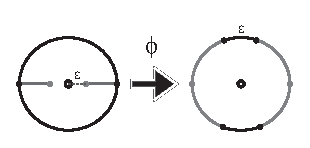
\includegraphics{conformal_map.eps}
\end{center}
\caption{The conformal map $\phi$ from $D$ to the unit circle}
\label{fig:conf_map}
\end{figure}

Our main result of this subsection is:
\begin{propos}\label{prop:confmain}
The conformal map above has:
$$\Re \phi(z) = -\frac{\epsilon}{1+\epsilon^2}\frac{1+z^2}{z},$$
for $z\in\mathbb{R}$ such that $\epsilon\le|z|\le1$.
\TODO{}{Need to say something about extending to the conformal
boundary}
\end{propos}
\begin{proof}
The main instrument in our proof is the explicit description of $\phi$.
We ease this description on the reader, by describing two
auxiliary functions, $G(z)$ and $H(z)$. We define $G(z)=\frac{1+z}{1-z}$
and $H(z)=\frac1{g(z)^2+g(-\epsilon)^2}$. We then define
\begin{equation}\label{eq:functionf}
\phi(z)=\frac{i\sqrt{H(\epsilon)-H(z)}-\sqrt{H(0)-H(\epsilon)}}{i\sqrt{H(\epsilon)-H(z)}+\sqrt{H(0)-H(\epsilon)}}
\end{equation}
\TODO{}{should we show that $\phi(z)$ is indeed the conformal map we are after?}
We can multiply \eqref{eq:functionf} by its numerator to calculate $\Re \phi(x)$, when $x$ is real. This calculation yields
\begin{equation}\label{eq:refunctionf}
\Re \phi(z)=\frac{H(0)-2H(\epsilon)+H(z)}{H(0)-H(T)}
\end{equation}
Expanding \eqref{eq:refunctionf}, and using the fact $\epsilon\le |z|\le1$ we get:
$\Re \phi(z) = -\frac{\epsilon}{1+\epsilon^2}\frac{1+z^2}{z}$ as required.
\end{proof}

The next couple of Corollaries will establish the unresolved parts of Proposition \ref{prop:trans}. Both will use the fact a Brownian motion has radial symmetry in the plane and thus its chance of leaving a circle through some arc is proportional to its length.

\begin{cor}\label{m22and23true}
Items \ref{m22} and \ref{m23} in Proposition \ref{prop:trans} are true.
\end{cor}
\begin{proof}
Denote by $u$ the length of each of the two arcs in the unit circle
which are the images of the arcs $1\frown-1$. By Proposition
\ref{prop:confmain} we have $\Re \phi(-1)=-\Re
\phi(1)=2\frac{\epsilon}{1+\epsilon^2}$. As the length of an arc in a
semicircle cannot exceed $\pi$ times the length of a string leaning on
it, we get $u \le \frac{4\pi\epsilon}{1+\epsilon^2} = O(\epsilon)$.
\end{proof}

\begin{cor}\label{m24true}
Item \ref{m24} in Proposition \ref{prop:trans} is true.
\end{cor}
\begin{proof}

In order to prove Item \ref{m24} in Proposition \ref{prop:trans}, we should calculate the length $u$ of the arc between $\phi(-r_0)$ and $\phi(-r_1)$.
%By Proposition \ref{prop:confmain} we have $\Re\phi(-r_i)=\frac{\epsilon}{1+\epsilon^2}\frac{1+r_i^2}{r_i}$ for $i\in\{0,1\}$.
%Since $r_0>2\epsilon$,
%$|\Re\phi(-r_1)-\Re\phi(-r_0)| \frac{\Re \phi (2\epsilon)}{ \sqrt {1-\Re \phi (2\epsilon)^2}} \le u$.

Notice that $\phi(r)$ lies on a semi-circle for $r\in[2\epsilon,1]$,
and that the slope of the semicircle is bounded from below (say by
$m$) on $\Re\phi([2\epsilon,1])$. This leads to the bound:
$|\Re\phi(-r_1)-\Re\phi(-r_0)| m \le u$.
On the other hand,
\[|\Re\phi(-r_1)-\Re\phi(-r_0)|
=
\frac{\epsilon}{1+\epsilon^2}\left|\frac{1+r_1^2}{r_1}-\frac{1+r_0^2}{r_0}\right|
\ge\epsilon\left(\frac1 {r_0} - \frac 1{r_1}-1 \right).\]

\end{proof}




}

%  {
  \section{Tom's versions of some results}

  Let $X$ be the process which is a two-dimensional Brownian motion,
  absorbed on the line $x = y$ when $x = y \ge \epsilon$ and released
  when $x = y = 0$.

  \newcommand{\radius}{\delta}

  We'd like to show that $X_1$ is within $\radius$ of the line with
  high probability.  In fact we will show that for all $t \in [0,1]$
  $X_t$ is within $\radius$ of the line with high probability.

  \newcommand{\twonorm}[1]{\|#1\|}

  Let $0 = S_0 > T_1 > S_1 > T_2 > S_2 > T_3 > S_3, \ldots$ be the
  largest collection of stopping times such that $X_{S_i} = 0$ and
  $\twonorm{X_{T_i}} = \radius$.

  Then there are exactly $k$ escapes-and-returns-to-$0$ by time $S_k$.

  Consider the probability of the event
  \[
  \text{Until time $S_k$ all the escapes are through the line, and
    $S_k \ge 1$}
  \]
  This is no smaller than the probability for the event
  \[
  \text{Until time $S_k$ all the escapes are through the line, and
    $\sum_{i=1}^k S_i - T_i \ge 1$}
  \]
  which is 
  \begin{multline*}
  \P\left(\sum_{i=1}^k S_i - T_i \ge 1 | \text{Until time $S_k$ all
    the escapces are through the line} \right) \\ \cdot \P(\text{Until time
      $S_k$ all the escapces are through the line})
  \end{multline*}
  which is
  \begin{multline*}
  \P(\text{Time for BM to go from $0$ to $k\radius \ge 1$})
  \\ \cdot \P(\text{A particular launch escapes through the
    line})^k
  \end{multline*}
  This is then a lower bound for the probability of
  \[
  \text{By time $1$ all the escapes are through the line}
  \]
  (this one is (a bit stronger than) what we want for Proposition
  \ref{thm:main2}) which itself is a lower bound for the probability
  of
  \[
  \text{At all times $t \in [0,1]$, $X_t$ is within $\radius$ of the line}
  \]
}

  {
\section{Conclusions about the noise}

Horizontal = noise

Rect factorization

2dim noise

\newcommand{\F}{\mathcal{F}}
A $d$-dimensional noise consists of a probability space $(\Omega,F, \P)$, sub-$\sigma$-fields $\F_R \subset \F$ given for
all (open) $d$-dimensional rectangles $R \subset \R^d$, and a measurable action $(T_h)_h$ of $\R^d$ on, having the following
properties:
\begin{enumerate}
\item \label{item:tensor-condition} $\F_R \tensor \F_{R'} = \F_{R''}$ whenever $R''$ is a
rectangle partitioned by rectangles $R$ and $R'$ in the sense that
$R\cap R'=\emptyset$ and the closure of $R \cup R'$
is the closure of $R''$,
\item \label{item:translation-condition} $T_h$ sends $\F_R$ to $\F_{R+h}$ for each $h \in \R^d$,
\item \label{item:generation-condition} $\F$ is generated by the union of all $\F_R$.
\end{enumerate}

In the case of a one-dimensional noise, $R$ ranges over all open intervals
and condition~(\ref{item:tensor-condition}) translates to
$\F_{(s,t)} \tensor \F_{(t,u)} = \F_{(s,u)}$ whenever $s < t < u$.

As conditions $\label{item:translation-condition}$ and
$\label{item:generation-condition}$ are immediate for
Horizontal factorization of the Brownian web (see
Definition~\ref{def:horizontal-factorization}),
Theorem~\ref{thm:recoveringfromstrips} immediately
implies the following:

\begin{theorem}
The Brownian web, factorized on horizontal strips is a noise.
\end{theorem}

We can also extend the definition of the horizontal
factorization of the web, defining a two-dimensional
factorization into rectangles along the lines of the
same definition. As the proof of Theorem \ref{thm:recoveringfromstrips}
holds when restricted to vertical strips, and the proof of its vertical
counterpart holds when restricted to horizontal strips (see \TODO{}{add
ref if possible}), we can extend our results to derive the following:

\[\text{The Brownian web, factorized on two-dimensional
rectangles is a two-dimensional noise.}\]

Furthermore, by a completely general and abstract result
of Tsirelson \TODO{}{cite}, a two dimensional noise which is
black in one of its one-dimensional factorizations, is also
black. As this holds for the Brownian web (see \TODO{cite}),
we end up with to following:

\begin{theorem}
The Brownian web, factorized on two-dimensional rectangles is a two-dimensional black noise.
\end{theorem}
%Hurra!

\TODO{\section{Open problems}}{This belongs in a different file, perhaps}

\TODO{\section{Acknowledgements}}{This belongs in a different file,
  perhaps}

\TODO{\begin{itemize}
\item Boris for discussion
\item Ron for significantly simplifying an earlier argument, for many helpful
  comments during writing
\item Nomi
\item anyone from Ohad?
\end{itemize}}{}
}

  \begin{thebibliography}{99}
\bibitem{fontes-et-al} L. R. G. Fontes, M. Isopi, C. M. Newman, and
  K. Ravishankar. The Brownian web: characterization and
  convergence. Ann. Probab., 32(4):2857--2883, 2004.
\bibitem{norris-turner-convergence-to-bw} James Norris and Amanda
  Turner. Planar aggregation and the coalescing Brownian flow.
  arXiv:math.PR/0810.0211, 2008.
\bibitem{norris-turner-planar-aggregation} James Norris and Amanda
  G. Turner. Planar aggregation and the coalescing Brownian
  flow. arXiv:math.PR/0810.0211, 2008.
\bibitem{toth-werner} Balint Toth and Wendelin Werner. The true
  self-repelling motion. Probab. Theory Related Fields,
  111(3):375--452, 1998.
\bibitem{tsirelson-nonclassical-stochastic-flows} Boris Tsirelson,
  Nonclassical stochastic flows and continuous products
  http://arxiv.org/abs/math/0402431v3
\bibitem{tsirelson-completion} Boris Tsirelson, Noise as a Boolean
  algebra of sigma-fields. I. Completion, http://arxiv.org/abs/1107.3042v2
\bibitem{tsirelson-classicality-blackness-spectrum} Boris Tsirelson,
  Noise as a Boolean algebra of sigma-fields. II. Classicality,
  blackness, spectrum
  http://arxiv.org/abs/1109.1690
\bibitem{billingsley} Billingsley 1999
\end{thebibliography}

}

\end{document}
